%\documentclass{report}
%\usepackage[T1]{fontenc}
%\usepackage[utf8]{inputenc}
%\usepackage[francais]{babel}
%\usepackage{amsmath}
%\usepackage{graphicx}
%\usepackage[backend=biber,style=authoryear,bibencoding=utf8]{biblatex}
%\usepackage[colorlinks,linkcolor=blue]{hyperref}
%
%\addbibresource{biblio.bib}
%

%\begin{document}
\chapter{L'actine}

L'actine est une protéine ubiquitaire conservée chez tous les eucaryotes, exprimée dans tous les types cellulaires. 
Ses fonctions sont multiples et variées et se divisent en deux catégories principales, les fonctions mécaniques et les fonctions régulatrices. 

Elle se présente dans la cellule sous deux formes principales : en monomères (Actine G pour globulaire) ou en filaments (Actine F). 
Elle interagit avec un grand nombre de protéines (certains pensent même qu'il s'agit de la protéine interagissant avec le plus grand nombre d'autres protéines) appelées Actin-Binding Proteins. 

L'actine est un composant du cytosquelette sous forme d'un réseau de filaments très dynamique. La rigidité d'une cellule et sa motilité sont majoritairement contrôlées par l'organisation du cytosquelette d'actine. 

Mais l'actine est également un composant des trois ARN Polymérases PolI, PolII et PolIII, qui transcrivent l'ADN en ARN pendant la première étape de l'expression du génome. 
Elle est indispensable à la réorganisation de la chromatine qui précède l'expression mais aussi à l'export de l'ARN.  

L'association de ces rôles mécaniques et biologiques fait de l'actine un acteur de choix dans l'interface entre les signaux mécaniques et les signaux biologiques. 

Dans le corps, l'actine a des fonctions spécifiques dans un grand nombre d'organes, comme la contraction des muscles, l'organisation des dendrites et des axones des neurones, le fonctionnement des plaquettes ou de l'appareil auditif. 



\section{Actine G}

\begin{figure}
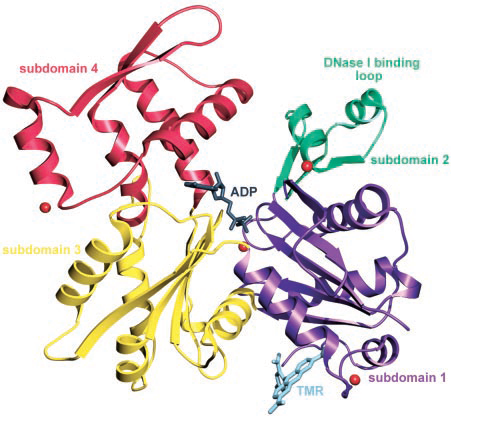
\includegraphics[scale=0.7]{Actine_dominguez.png}
\caption{Cristallisation d'un monomère d'actine ADP, d'après \cite{otterbein_crystal_2001}}
\end{figure}

Chez les mammifères, l'actine est codée par 6 gènes qui peuvent donner une trentaine de molécules différentes par le jeu de l'épissage. 
Elles sont divisées en trois familles : les actines $\alpha$ qui sont exprimées dans les muscles cardiaques, lisses et squelettiques, les actines $\beta$ et $\gamma$ exprimées dans les autres types cellulaires.
Les différentes formes d'actine sont très proches en séquence, mais ne peuvent pas complètement se substituer les unes aux autres. Toutes les formes peuvent s'incorporer dans les filaments. 

La protéine transcrite a un poids moléculaire de 42 kDa, et est produite en grande quantité dans les cellules, où elle pèse environ pour 1 à 5 \% de la masse protéique. 

\subsection{Structure}
La structure moléculaire de l'actine a été observée un grand nombre de fois, en cristallisation avec différents ABP comme la Dnase, la latrunculine ou la profiline. 


Elle est composée de 4 sous-domaines organisés en deux lobes. Les sous-domaines 2 et 4 forment l'extrémité - du filament, les sous-domaines 1 et 3 forment l'extrémité +. Entre les deux lobes se trouve le site de liaison à l'ATP. 
À côté de ce site se trouve une zone d'interaction avec les cations divalents (Ca$^{2+}$ ou Mg$^{2+}$). 

Dans le sous-domaine 2 se trouve une structure de 8 acides aminés appelée Dnase binding loop, désorganisée dans la plupart des cristallisations de l'actine mais organisée en feuillet $\beta$ lorsqu'elle est liée à la Dnase. Au centre de cet élément se trouve une méthionine en position 44 qui peut être oxydée par la protéine MICAL. 

\subsection{L'actine est une ATPase}

L'actine, après sa fabrication, n'est prête à jouer son rôle qu'avec l'ajout d'une ATP au centre de sa structure.
En plus de ses deux formes, globulaire ou filamenteuse, l'actine a donc également deux états énergétiques : ATP ou ADP.

Les deux formes d'actine, ATP et ADP sont capables de former des filaments et de s'incorporer à des filaments. 
Cependant, l'actine ATP est plus facilement polymérisée alors que l'actine ADP est plus facilement dépolymérisée. 
Les actines ATP incorporés dans un filament sont ensuite hydrolysées, et deviennent donc plus facilement dépolymérisables, ce qui donne lieu à un tapis roulant : les monomères s'ajoutent à un bout et s'enlèvent à l'autre. 

\subsection{Localisation et transport}

L'actine a longtemps été étudiée pour son rôle dans le cytoplasme, en tant que composant du cytosquelette. Cependant de l'actine est également présente dans le noyau de la cellule, où elle a des rôles essentiels. 
L'actine peut polymériser dans les deux compartiments, bien que l'on ne trouve pas de grands filaments organisés dans le noyau. 

L'actine est à une taille intermédiaire pour les pores nucléaires : elle n'est pas tout à fait assez petite pour diffuser facilement à travers. Elle est donc transportée activement entre le noyau et le cytoplasme. 
Son import nécessite la liaison à la cofiline, et est médiée par l'importine 9. Son export nécessite la profiline et est médiée par l'exportine 6. 



\subsection{Oxydation de l'actine}

Les protéines MICAL sont capables d'ajouter deux atomes d'oxygène sur la Met44 de l'actine. Cet acide aminé est au centre d'une zone de la protéine qui relie les monomères dans un filament. 
L'oxydation spécifique de cet acide aminé déstabilise les filaments et l'actine oxydée est incapable de se lier à d'autres actines pour former de nouveaux filaments. 

MICAL2 est une version de cette protéine localisée dans le noyau. L'actine qu'elle oxyde, en plus d'être dépolymérisée, est expulsée du noyau et ne peut plus y entrer. MICAL2 organise donc la régulation de l'actine nucléaire en appauvrissant le réservoir d'actine nucléaire en filaments et en monomères.

\subsection{Protéines interagissant avec l'actine G}

 La profiline est une petite protéine (autour de 15kDa) qui peut se lier à l'actine G par son extrémité +, l'empêchant de former un nouveau filament ou de se lier à l'extrémité - d'un filament existant. 
Bien qu'elle se lie au monomère, son action est globalement favorable à la croissance des filaments. 
La profiline facilite le remplacement d'une ADP par une ATP dans le monomère auquel elle est attaché. 
Or l'actine ATP polymérise mieux que l'actine ADP, l'action de la profiline va donc recycler l'actine ADP dépolymérisée des anciens filaments en actine ATP prête à allonger de nouveaux filaments. 
De plus, les élongateurs de filaments comme les formines et VASP vont préférentiellement utiliser de l'actine liée à la profiline pour faire croître les filaments. 
La profiline joue également un rôle dans la localisation de l'actine : l'exportine 6 va se lier spécifiquement au complexe actine-profiline et le faire passer de l'intérieur vers l'extérieur du noyau. 


Les thymosines $\beta 4$ sont de toutes petites protéines d'environ 5kDa dont le rôle principal est de maintenir un réservoir d'actine monomérique. Elles se lient principalement aux actines ATP et les empêchent de polymériser. 

Les CAP (Adenylate Cyclase Associated Protein) sont également des catalyseurs de l'échange une ADP contre une ATP dans les monomères d'actine. 

Les cofilines sont une famille de petites protéines qui lient à l'actine G et à l'actine F. Elles sont une préférence pour l'actine ADP. 
Le complexe cofiline-actine est plus facilement recruté par les CAP, qui vont  dissocier le complexe et remplacer l'ADP par une ATP sur l'actine. 
Les cofilines sont suffisamment petites pour passer par les pores nucléaires par diffusion, elles sont cependant dotées d'un signal de localisation nucléaire. Cela leur permet d'être importées dans le noyau lorsqu'elles sont liées à d'autres protéines plus massives. 
Ainsi, le complexe cofiline-actine est importé dans le noyau par l'importine 9. 

L'actine bloque l'activité de la DNase I, une enzyme qui coupe l'ADN en fragments de 4 paires de bases de manière non spécifique. La DNase I se lie à l'actine globulaire avec une grande affinité, alors qu'elle ne se lie que très peu à l'actine F, c'est pourquoi elle est souvent utilisée pour la détection de l'actine G en immunofluorescence. 

Les Myocardin-Related Transcription Factors sont des cofacteurs de transcriptions qui peuvent former un complexes avec trois ou cinq monomères d'actine. Leur rôle n'est pas de réguler l'équilibre dynamique de l'actine mais d'agir comme un détecteur de la concentration de monomères d'actine disponibles. 
En fonction de l'état de polymérisation du cytosquelette, les MRTF vont réguler l'activité d'un facteur de transcription contrôlant les gènes de l'actine et d'un grand nombre d'ABP qui régulent sa dynamique. 
Les MRTF sont un maillon d'une boucle de rétro-action qui contrôle la dynamique de l'actine à long terme par l'expression des gènes. 
Les mécanismes détaillés de ce contrôle et ses conséquences seront décrits dans un chapitre dédié. 

\section{Actine F}

La principale fonction de l'actine chez les eucaryote est sa capacité à former un réseau de filaments branchés, connecté par des moteurs moléculaires. 
La formation de filaments d'actine est régulée par de très nombreuses protéines qui vont se lier aux monomères ou aux filaments. 

\begin{figure}
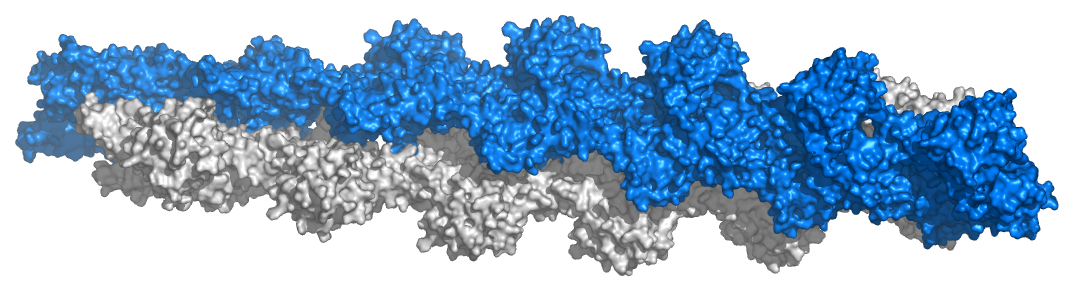
\includegraphics[scale=0.3]{Actin_filament_atomic_model.png}
\caption{Structure d'un filament d'actine basée sur le modèle de Ken Holmes, illustré par Thomas Splettstoesser}
\end{figure}

\subsection{Le filament}

Les filaments d'actine sont très dynamiques, et ont une structure changeante. Ils ont un diamètre de 6nm et une longueur de persistance de l'ordre de la dizaine de microns, donc du même ordre de grandeur que la taille typique cellulaire. 

Les monomères d'actine s'associent les unes à la suite des autres, l'extrémité pointue d'un monomère se liant à l'extrémité barbée de l'autre, avec une rotation entre un monomère et l'autre. 
Le filament est alors polarisé, avec une extrémité pointue notée également - et une extrémité barbée notée +. 

Les deux bouts du filaments ont des affinités différentes pour les monomères. En présence d'une grande quantité de monomères disponibles, le filament peut croître par les deux bouts, mais dans une concentration intermédiaire, le filament va croître par ajout de monomères à son extrémité + et décroître par dépolymérisation à l'extrémité -. L'équilibre entre les deux cinétiques de réaction détermine si la taille du filament croît ou non. 

Cet équilibre est connu comme le "tapis roulant" de l'actine : lorsque les deux cinétiques sont égales, le filament avance par remplacement des monomères en gardant une longueur constante. 

Bien que cet assemblage puisse avoir lieu spontanément en présence d'actine, de nombreuses protéines aident à la nucléation des filaments, à leur stabilité ou à leur déstabilisation. 

\subsection{L'équilibre de polymérisation}

Des protéines vont réguler toute l'existence d'un filament d'actine : la nucléation, la croissance, la stabilisation et la dissociation. 

\subsubsection{Les nucléateurs}
Les dimères et les trimères d'actine sont des structures peu stables, à la durée de vie assez courte. C'est à partir du tétramère que la structure devient suffisamment stable pour créer un nouveau filament d'actine. 

Afin de dépasser cette barrière, d'autres protéines jouent le rôle de nucléateurs. Le complexe Arp2/3 (Arp pour Actin Related Protein) est le plus connu de ces nucléateurs. Il se lie au côté d'un filament et Arp2 et Arp3 miment un dimère d'actine. D'autres monomères peuvent alors se fixer sur cette base et un nouveau filament peut croître. Ce nouveau filament est de plus attaché avec un angle fixé au filament initial, créant un réseau branché. 

Les formines se fixent à l'extrémité barbée d'un filament et y ajoutent successivement des monomères d'actine. Les formines peuvent nucléer un nouveau filament en stabilisant un dimère et en y ajoutant d'autres monomères. 

\subsubsection{Les élongateurs}

Une fois les filaments formés, des facteurs d'élongation comme les formines ou Ena/VASP, peuvent ajouter des monomères liés à la profiline à l'extrémité barbée du filament. 
Certaines formines avancent le long du filament tout en le construisant à partir de complexes actine-profiline. 


\subsubsection{Protéines de coiffage (capping proteins)}

Il existe deux sortes de protéines de coiffage : celles qui se lient à l'extrémité barbée et contribuent donc à réduire la polymérisation (comme CapZ, la gelsolin ou la tensine), et celles qui se lient à l'extrémité pointue, empêchant la dépolymérisation (comme la tropomoduline). 


\subsubsection{Protéines de fragmentation (severing proteins)}
Les protéines de frangmentation découpent et dépolymérisent les filaments d'actine. 

La cofiline se lie aux filaments d'actine ADP et entraîne une configuration où la rotation des monomères les uns par rapport aux autres est plus grande. Cela déstabilise les filaments et les casse. 

La gelsoline et la famille des villines et la fragmine sont également des facteurs de dépolymérisation des filaments d'actine. 

À première vue, on peut voir l'impression que ces protéines vont avoir tendance à diminuer le nombre et la longueurs des filaments et participer à la destruction du cytosquelette. Cela peut être le cas, mais pas toujours : la fragmentation d'un long filament en de nombreux filaments courts fait apparaître de nombreuses extrémité barbées là où il n'y en avait qu'une seule. Selon les conditions, en particulier l'activation de facteurs d'élongation et la disponibilité des monomères, la fragmentation peut donc agir en faveur de la polymérisation, en particulier lors du remplacement d'un réseau à longs filaments par un réseau très dense et réticulé. 

Les protéines MICAL sont une nouvelle famille de protéines dépolymérisant l'actine, découvertes dans les neurones. En oxydant l'actine des filaments, elle les dépolymérise. Comme l'actine oxydée ne peut plus former de nouveaux filaments, la destruction du cytosquelette par MICAL ne peut pas promouvoir la croissance du réseau. 

\subsubsection{Stabilisateurs des filaments}

Les tropomyosines sont des protéines qui vont former également des filaments. Ces filaments vont s'enrouler autour des filaments d'actines et les protéger : ils bloquent l'activité des cofilines et avec la troponine ils promeuvent l'association avec les myosines. 

Les nébulines sont des protéines stabilisantes dont le but est de fixer la longueur du filament d'actine auquel elles vont se lier, à la manière d'un étalon de mesure. 

\begin{figure}[h!]
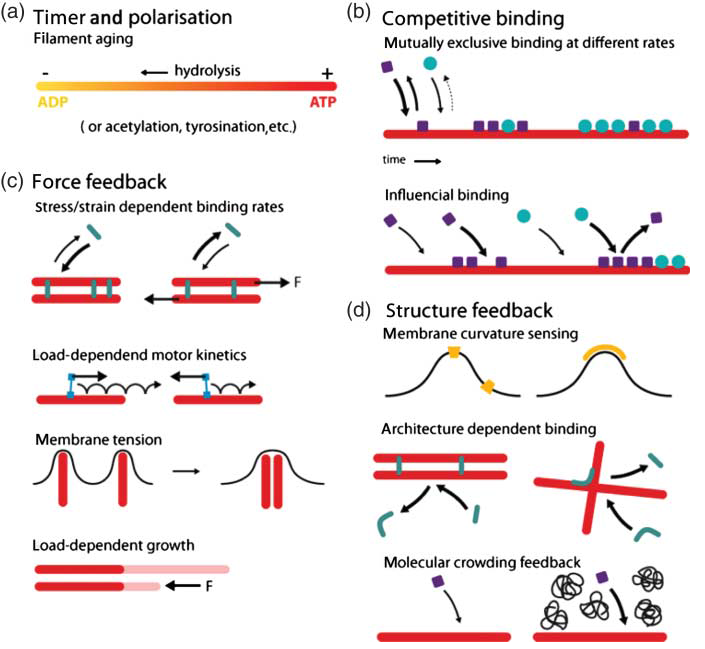
\includegraphics[scale=0.7]{Actine_phenomenon.png}
\caption{•}
\end{figure}

\subsection{Organisation en réseau de filaments}

Les filaments d'actine en évolution permanente sont liés entre eux par des protéines de pontage, liés à la membrane plasmique et liés aux autres filaments du cytosquelette (microtubules et filaments intermédiaires). 

\subsubsection{Ancrage à la membrane}

Les cellules sont liées mécaniquement entre elles par les cadhérines qui relient leur réseau d'actine. Les caténines font la liaison entre les cadhérines et les filaments d'actine. 

L'ancrage du cytosquelette à la matrice extra-cellulaire se fait par l'intermédiaire d'une structure extraordinairement complexe, les adhésions focales. 
Au niveau des adhésions focales, des dizaines de protéines interagissent entre elles pour relier les intégrines enchâssées dans la membrane et les filaments d'actine. 
Il serait impossible de faire ici l'inventaire des protéines impliquées dans ces adhésions. 
À l'intérieur des adhésions focales, une signalisation complexe est à l'\oe uvre qui permet, en réponse à des forces extérieures, de construire une structure mécanosensible capable de déclencher des cascades de signalisation dans toute la cellule. 
En particulier, les petites GTPases Rac, Rho et Ras sont activées par les adhésions focales soumises à des signaux mécaniques et régulent l'architecture du cytosquelette. 

\subsubsection{Protéines de pontage}

Les filaments d'actine sont organisés en réseau par des protéines comme la filamine, la spectrine ou la transgeline. 

La filamine est un homodimère qui lie deux filaments d'actine. Elle peut se déformer sous la contrainte, ce qui permet doter le réseau d'actine à la fois d'une élasticité et d'une mécanosensibilité supplémentaire.
La filamine peut également se lier à la membrane pour y ancrer le réseau d'actine. 

Les tétramères de spectrine s'associent à l'actine pour former un réseau hexagonal soutenant la membrane plasmique. 


\subsubsection{Protéines de faisceau}

Ces protéines permettent de rassembler les filaments d'actine en faisceaux parallèles ou anti-parallèles. Cette architecture est retrouvée dans les filopodes, dans les fibres de stress ou dans les microvillosités.

Il peut y avoir deux domaines de liaison à l'actine sur la même protéine, comme c'est le cas pour la fimbrine, l'écart entre deux filaments est alors faible et le faisceau maintenu serré. 
Des protéines se liant à l'actine peuvent également former des dimères ou des multimères où chaque sous-unité lie un filament. L'$\alpha$-actinine permet ainsi de former des fibres de filaments anti-parallèles. La jonction entre les filaments est plus souple et moins serrée. 

\subsubsection{Lien avec les autres filaments du cytosquelette}

Le cytosquelette d'actine est relié aux réseaux de filaments intermédiaires et aux microtubules par des protéines capables de se lier aux trois types de filaments. 
Par exemple, la plectine et les nesprines permettent de connecter les microtubules et les filaments d'actine au réseau de lamines de la membrane nucléaire, et donc de transmettre les contraintes jusqu'au noyau. 

 



\subsubsection{Moteurs moléculaires : myosines}

Les myosines sont des moteurs moléculaires qui se déplacent sur l'actine en consommant de l'ATP. Il en existe chez tous les eucaryotes, mais leur homologie n'est pas aussi grande que celle de l'actine, car elles ont des fonctions différentes. Dans le génome humain, on dénombre une quarantaine de gènes pour la myosine. 

La myosine II, aussi appelée "conventionnelle" est la plus étudiée. Elle est présente en quantité importante dans le muscle, car avec l'actine elle permet la contraction musculaire. 

Les myosines ont une tête qui peut se lier à l'actine en filament, un cou  qui sert de levier et de régulateur, et une queue qui sert souvent à former un dimère, et éventuellement à se lier à un cargo. On les appelles "chaînes lourdes" par opposition aux "chaînes légères", qui ne sont pas à proprement parler des myosines mais qui sont des protéines qui vont se lier au cou des "chaînes lourdes" pour les réguler. 

Par exemple, pour la contraction musculaire, deux chaînes lourdes de myosine II s'associent en dimère par leur queue, et quatre chaînes légères s'ajoutent au niveau des deux cous. Le dimère a alors deux têtes pouvant se lier à l'actine, et va s'en servir comme de deux jambes pour avancer le long du filament. 
La myosine est une ATPase, lors de l'hydrolyse de l'ATP qui lui est attachée, sa tête va changer de conformation et se détacher de l'actine. L'ADP sera alors libérée, et remplacée par une nouvelle ATP.  La tête reprend alors sa conformation initiale, et peu se rattacher au filament. Dans le dimère, chaque tête va faire ainsi un pas successivement et faire avancer le moteur sur le filament en consommant de l'ATP. 



Certaines myosines ont un rôle analogue à celui des moteurs moléculaires associés aux microtubules et transportent des molécules le long des filaments, en général en direction de l'extrémité + (seule la myosine VI se déplace en sens inverse). 


Les faiceaux anti-parallèles peuvent être liés par des paires de dimères, qui vont marcher en sens opposé sur les deux filaments, et donc les déplacer l'un par rapport à l'autre. Si les deux filaments sont liés par ailleurs dans le réseau, il va être mis sous tension par ces moteurs moléculaires.

\begin{figure}
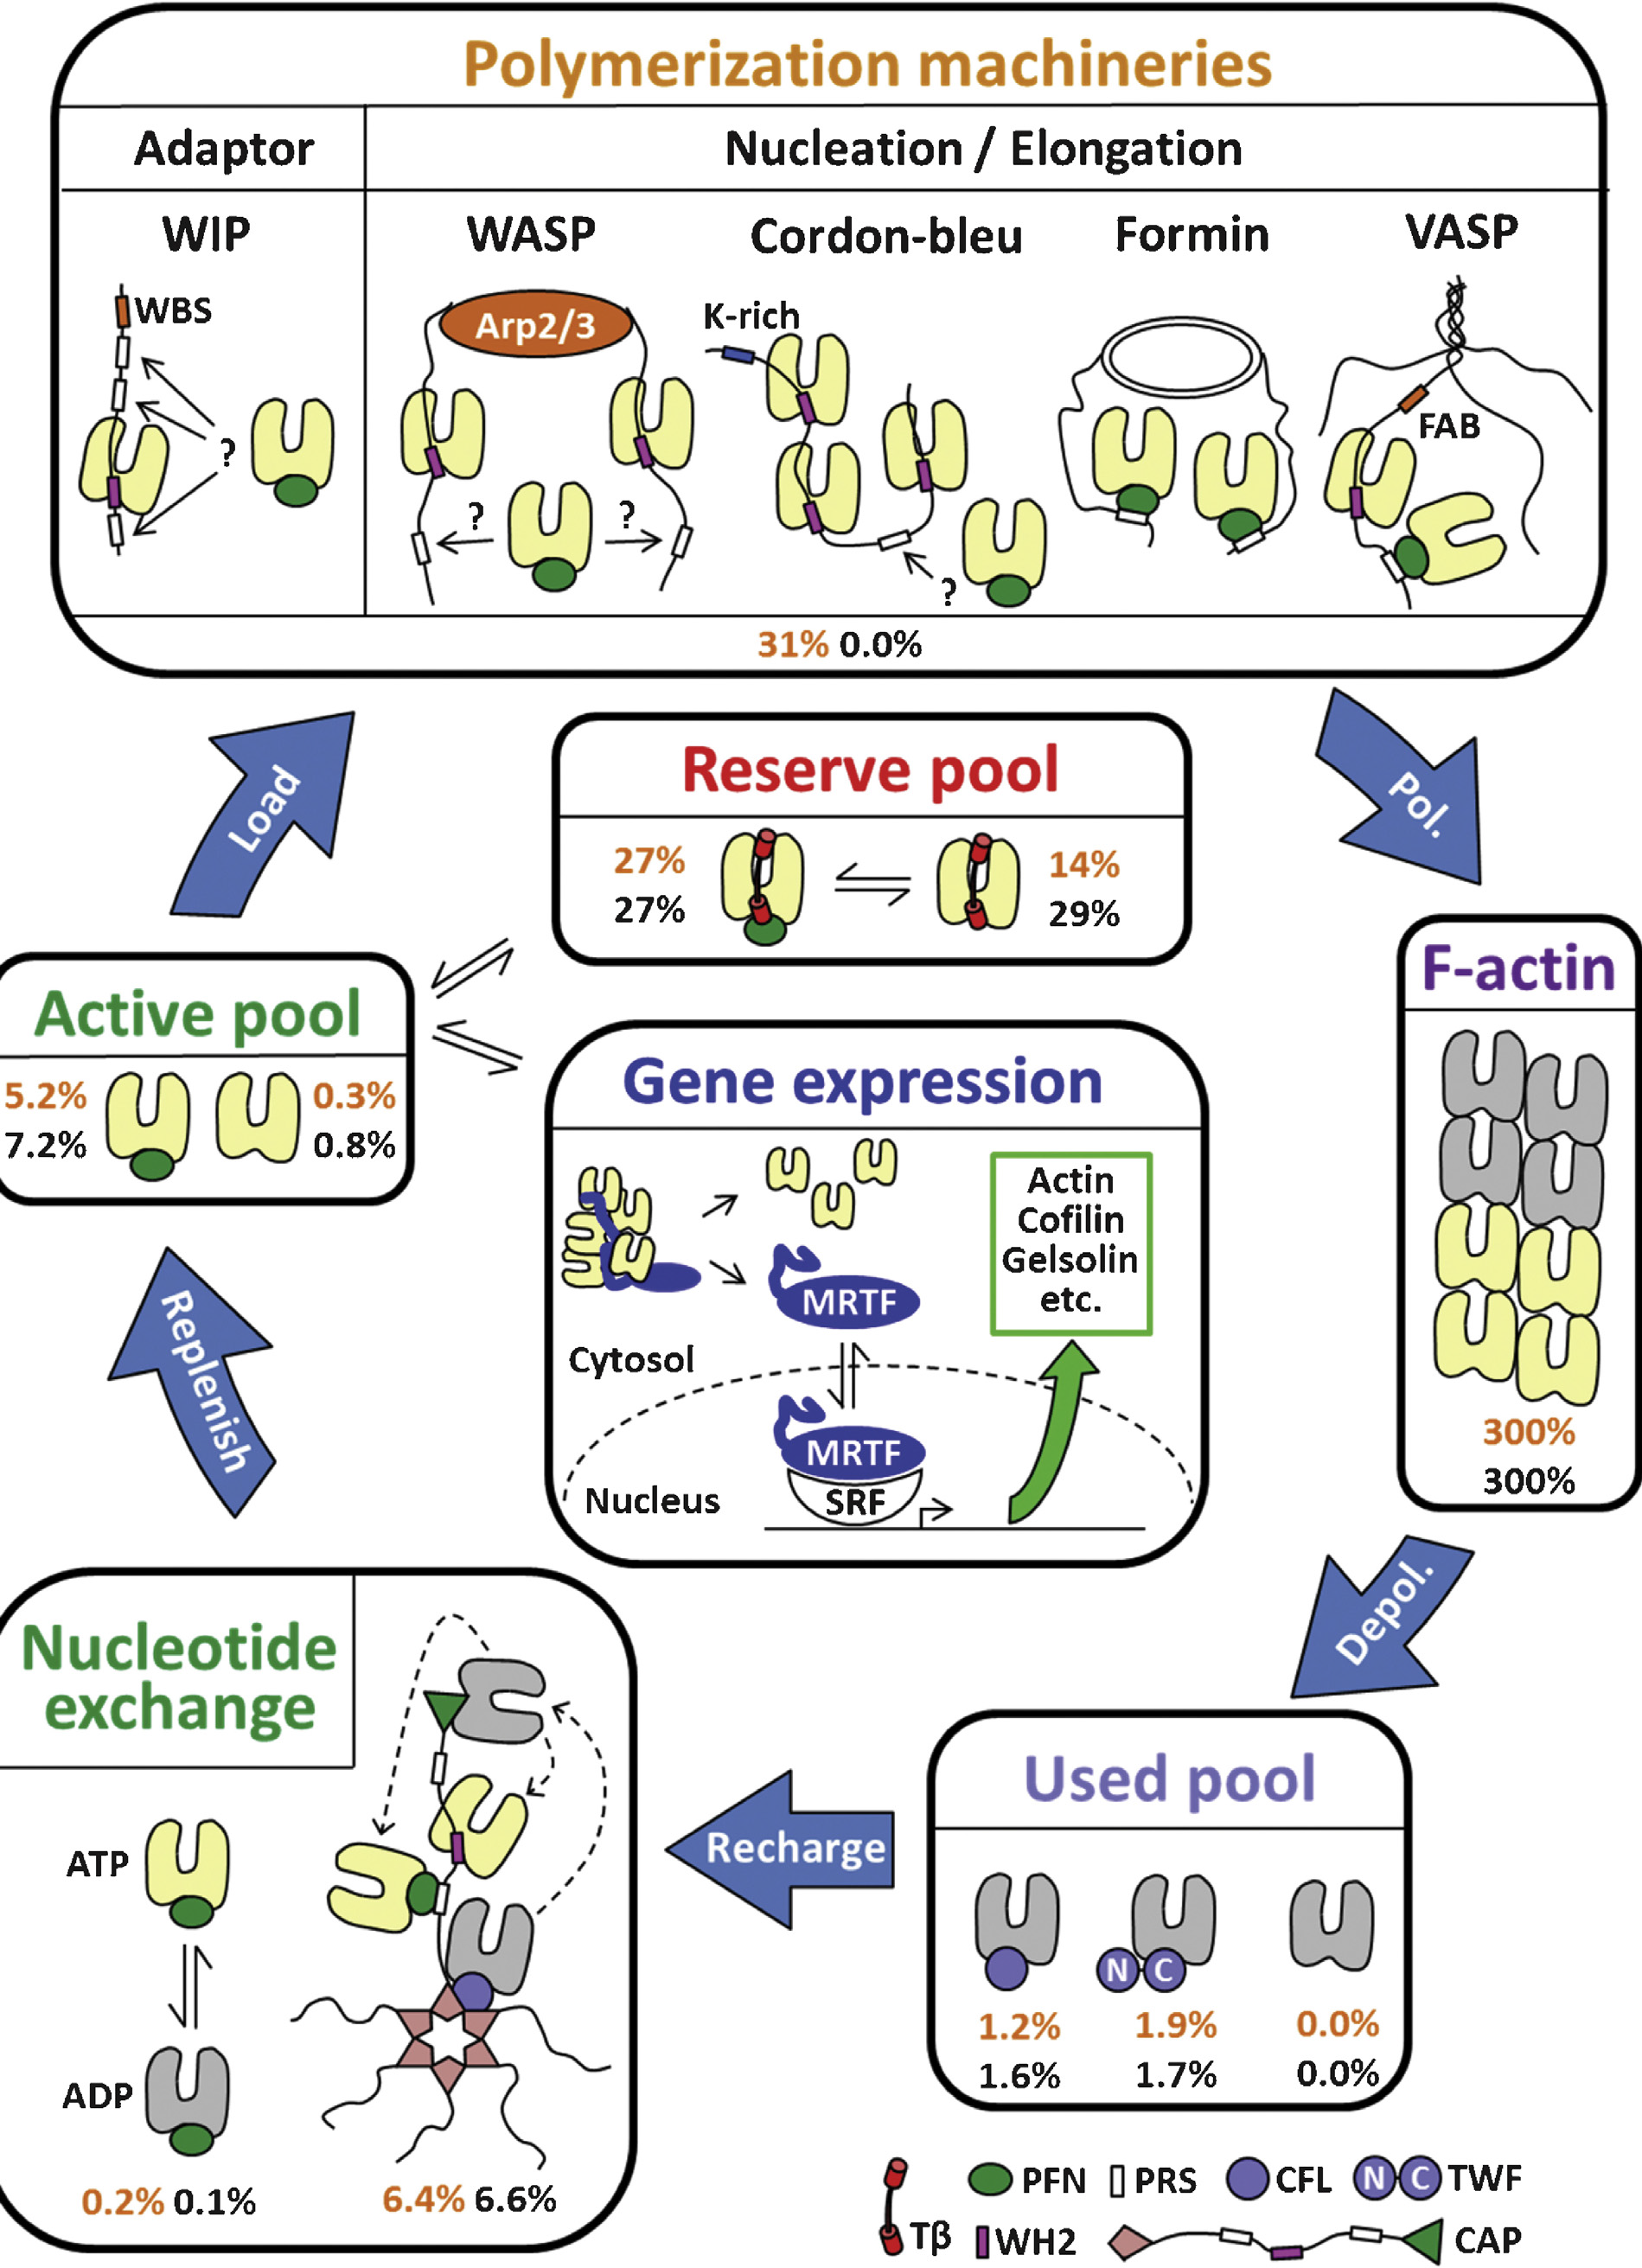
\includegraphics[scale=0.25]{actine_cycle.png}
\end{figure}


\section{Rôle mécanique de l'actine : du filament au cytosquelette}

Le cytosquelette est une structure multi-échelle, allant de l'échelle des moteurs moléculaires et des nucléateurs, à l'échelle de la cellule toute entière, en passant pas l'échelle des filaments et des réseaux de filaments. Il peut ressentir et exercer des forces à toutes les échelles. 


Dans cette partie, il ne s'agit pas de parler des propriétés mécaniques du cytosol ou de la cellule, mais d'expliquer comment les filaments peuvent générer des forces et comment il réagissent à des forces. 

\subsection{Mécanique du filament d'actine}

Le filament d'actine en lui-même est à la fois générateur et senseur de forces. 

 \subsubsection{Longueur de persistance}
La longueur de persistance est un moyen de quantifier la corrélation entre l'orientation des différents segments d'un polymère soumis aux fluctuations thermiques. Si l'on considère un polymère de longueur $L$ auquel on attribue une abscisse curviligne $s$, avec $\vec{t_s}$ la tangente au polymère en $s$, alors on a la relation : 
$$ \langle \vec{t_0}\cdot \vec{t_s} \rangle_L \propto e^{L/\ell_p}$$

Au bout de quelques longueurs de persistance, l'information de l'orientation du polymère en $s=0$ est perdue. 

La longueur de persistance dépend de l'énergie thermique disponible pour agiter le filament. Une manière de définir la rigidité d'un polymère indépendamment de la température consiste à définir un module de courbure comme le produit de la longueur de persistance et de l'énergie thermique : $$\kappa = \ell_p k_B T$$


Le filament d'actine subit un vieillissement par l'hydrolyse de l'ATP des monomères qui le composent. Le changement de conformation induit par l'hydrolyse de l'actine a des conséquences sur les propriétés mécaniques du filament. 
Un filament d'actine ATP a une longueur de persistance de 15 micromètres, contre 9 micromètres pour un filament d'actine ADP. Le vieillissement du filament le rend donc plus déformable et plus souple. 
Les protéines attachées au filament peuvent également, en stabilisant une conformation, changer sa rigidité. Un filament stabilisé par la phalloïdine ou par la tropomyosine voit sa longueur de persistance augmentée à 18 et 20 microns respectivement. Au contraire, la conformation stabilisée par la cofiline n'a qu'une longueur de persistance de 2,2 microns. 

Un même filament d'actine peut évidemment être le lieu de toutes ces modifications en même temps. Souvent l'extrêmité + des filaments est riche en actine ATP alors que l'extrémité - est riche en actine ADP, ce qui crée un filament plus rigide d'un côté et plus flexible de l'autre. 

\subsubsection{Couplage traction-torsion}

L'hélice que forme le filament peut adopter des conformations différentes, en particulier en ce qui concerne l'angle de rotation entre les monomères successifs. 
Une force tirant sur le filament va alors favoriser une conformation à faible torsion, ce qui va rendre la fixation de la cofiline, qui stabilise le filament dans une conformation à grande rotation, beaucoup plus difficile. 
Il en résulte que la cofiline est moins efficace sur les filaments qui sont en tension, induisant une préservation automatique des filaments sous contrainte par rapport aux filaments libres. 
Au contraire, mDia1 et la profiline sont plus efficaces sur les filaments soumis à une tension. 
La conformation de l'actine est alors un senseur de contrainte qui va encourager la préservation et l'élongation des filaments qui ressentent une force de traction. 

Les filaments d'actine semi-flexibles peuvent également être courbés, en particulier au voisinage de la membrane. 
À cause de l'organisation hélicoïdale des monomères, la courbure d'un filament d'actine exerce également une torsion sur ce filament, ce qui rend la modélisation des filaments encore plus complexe. 
Le facteur de nucléation Arp2/3 se lie plus facilement au côté convexe d'un filament d'actine courbé. 

\subsubsection{Les myosines}

L'action mécanique de la tête de myosine sur le filament d'actine se fait par un changement de conformation à l'échelle de la protéine. 
La myosine ayant hydrolysé son ATP en ADP + phosphate s'est liée à l'actine. Elle va alors changer de conformation en libérant le phosphate puis l'ADP. 
Cette dernière étape transforme l'énergie chimique de l'ATP en déplacement mécanique sur le filament d'actine. 
À l'ajout d'une nouvelle ATP, la myosine se détache. 

Ces évènements sont eux-même dépendant des contraintes qui peuvent être appliqués à la myosine. 
L'application d'une force de 1,6pN poussant la myosine vers sa conformation finale divise par deux la durée que la myosine va passer attachée au filament en facilitant le changement de conformation. 
Inversement, l'application de la même force en sens opposé multiplie par deux la durée d'attachement. 
En fait, la durée que la myosine passe attachée au filament d'actine dépend exponentiellement de la force exercée, dans la gamme -2pN $-$ 2pN. 




\subsection{Mécanique des adhésions focales}

Les sites d'ancrage de la cellule dans la matrice extra-cellulaire sont la porte d'entrée des signaux mécaniques dans la cellule. Parmi les molécules qui constituent les adhésions focales, certaines réagissent directement lorsqu'elles sont soumises à des stimulations mécaniques. 

Lorsque la transmission des forces est coupée dans la cellule (par l'ajout de drogues qui inhibe la contractilité du cytosquelette), les adhésions focales disparaissent : la tension est nécessaire non seulement à leur constitution, mais également à leur maintien. Ces contraintes peuvent provenir de forces extérieures mais aussi de la contraction du cytosquelette sous l'action des moteurs moléculaires. 

\begin{figure}
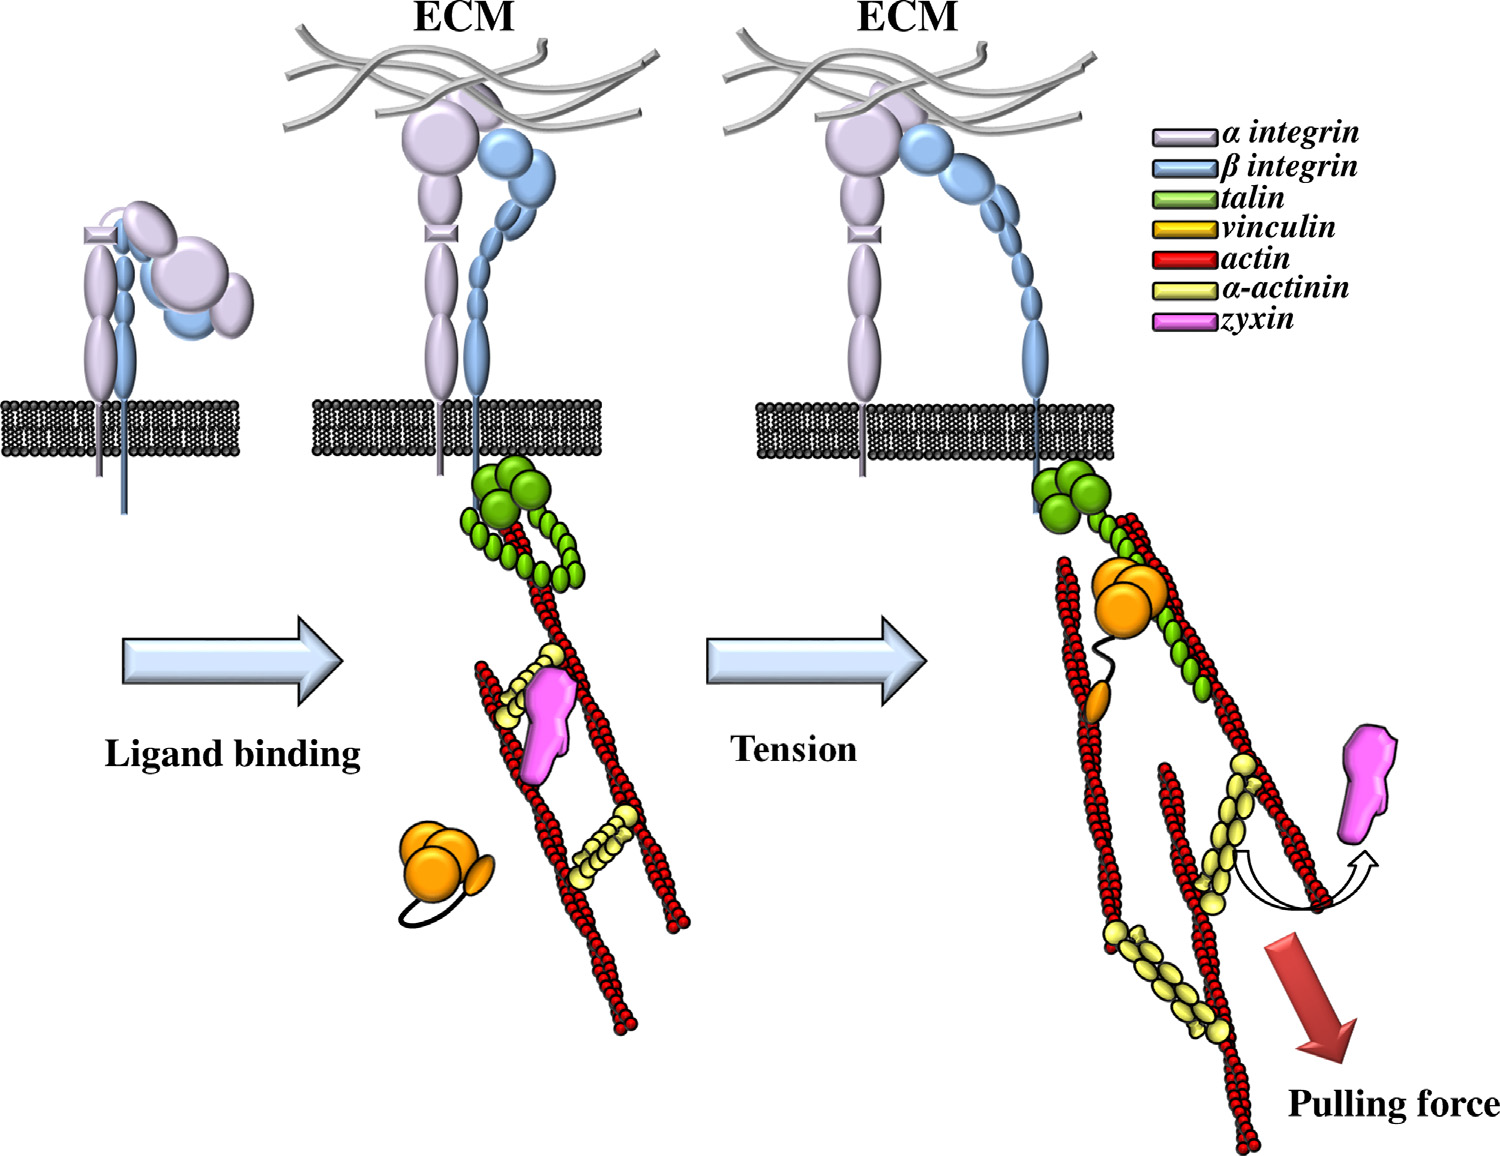
\includegraphics[scale=0.2]{Focal_adhesions_taline.png}
\end{figure}

En présence d'une force, les intégrines forment des agrégats et leur affinité pour le ligand augmente grâce à un changement de conformation. 
La taline relie les intégrines aux filaments d'actine. Dans la conformation initiale, elle est repliée sur elle-même. Lorsqu'elle est mise sous tension entre les intégrines et l'actine, elle se déplie, laissant apparaître des domaines de liaisons à la vinculine qui n'étaient pas précédemment accessibles. 
La vinculine peut alors recruter d'autres protéines dans les adhésions focales, comme l'$\alpha$-actinine, qui connecte les filaments d'actine en faisceaux. L'étirement de l'$\alpha$-actinine change sa configuration et pourrait être à l'origine de la relocalisation de la zyxine en réponse aux contraintes mécaniques. 

La filamine, qui lie entre eux des filaments d'actine, peut être dépliée lors de tensions sur les filaments. Son domaine de liaison aux intégrines devient alors accessible, et la filamine ancre alors le cytosquelette à la matrice extra-cellulaire par l'intermédiaire des intégrines. De plus, cela cause un changement de conformation des intégrines qui favorise la formation d'agrégats, renforçant l'adhésion. 

Ce ne sont là que quelques exemples de protéines impliquées dans les adhésions focales, il en existe des centaines. Leur exemple montre qu'au premier niveau de contact avec l'environnement mécanique extérieur, les forces sont transcrites en signal biologique au niveau de la molécule individuelle, en changeant la conformation des protéines. 



\subsection{Mécanique du cytosquelette d'actine}

\section{Rôle régulateur de l'actine nucléaire}

L'actine nucléaire est plus difficile à observer que l'actine cytoplasmique, c'est pourquoi son existence et son rôle ont été ignorés pendant longtemps. 
Aujourd'hui, l'amélioration des techniques de microscopie et le développement de techniques spécifiques (comme des sondes dotées d'un NLS) permettent de confirmer l'existence d'actine nucléaires tant en monomères qu'en filaments. 
De plus, un grand nombre de protéines liées à l'actine, comme la profiline, la cofiline, Arp2/3, N-WASP, les formines, MICAL et des myosines, sont également présentes dans le noyau, créant toutes les conditions pour qu'un véritable nucléosquelette soit constitué dans la cellule. 
La profiline et la cofiline aident respectivement à l'export et à l'import des monomères d'actine par les pores nucléaires, jouant ainsi un double rôle de régulation de l'actine nucléaire. 


\subsection{L'actine G nucléaire dans les complexes}

80\% de l'actine nucléaire est sous forme de monomères. Ces monomères vont d'incorporer dans un grand nombre de complexes indispensables à la transcription de l'ADN en ARN et à la maturation de l'ARN. 

Chez les eucaryotes, la transcription de l'ADN en ARN est effectuée par trois ARN Polymérases. Il a été montré que l'actine est nécessaire à l'activité des trois ARN Polymérases. Elle fait partie du complexe pré-initiation de l'ARN Poymérase II qui transcrit les gènes codant pour des protéines en pré-ARN messagers.

L'actine est également liée aux ribonucléoprotéines hétérogènes (hnRNP) présentes sur les pré-ARN messagers pendant et après leur transcription. Les hnRNP empêchent ces ARN messagers qui doivent encore subir des étapes de maturation de se replier sur eux-mêmes (ce qui pourrait interférer avec leur traitement) ou d'être exportés avant d'avoir été traités. Elles peuvent également se lier à la machinerie d'épissage. 

Les complexes de remodelage de la chromatine font passer la chromatine d'un état très compact impossible à transcrire à un état où l'expression des gènes devient possible. L'actine fait partie de plusieurs types de complexes de remodelage de la chromatine comme SWI/SNF, RSC et BAF. 

L'actine monomérique bloque également l'activité de la DNase I dans le noyau et l'empêche de couper l'ADN en petits morceaux. 

\subsection{Les filaments d'actine et la myosine nucléaires}

20\% de l'actine nucléaire est présente sous la forme de filaments. Les nucléateurs comme Arp2/3 et les formines sont présents dans le noyau, aux côtés d'élongateurs spécifiques comme l'émerine. 
Des myosines, comme la Nuclear Myosin 1 (NM1) et la myosine VI sont présentes dans le noyau et ont un rôle essentiel dans la transcription. 

L'actine, mais également N-WASP et Arp2/3 sont nécessaires à la transcription efficace par l'ARN Polymérase II. Les drogues empêchant la formation de filaments comme la latrunculine ou la cytochalasine D perturbent la transcription par PolII. La myosine VI s'associe également à PolII. 

La NM1 et l'actine se lient à PolI pour la transcription des gènes ribosomaux. La NM1 remodèle localement la chromatine dans une conformation favorable à la transcription. 

L'émerine, qui relie des filaments d'actine aux lamines qui enveloppent le noyau, joue un rôle essentiel dans l'organisation de l'hétérochromatine. 

Les myosines nucléaires sur le réseau d'actine sont capables de réorganiser les locus de gènes présents sur des chromosomes différents mais partageant un même promoteur. Par exemple, la translocation dans le noyau des récepteurs des hormones stéroïdiennes androgènes et \oe strogènes provoque le regroupement des sites des gènes cibles d'une manière active et dépendante de l'activité de l'actine et de la myosine nucléaire 1. 

Le noyau contient tous les éléments nécessaires à la formation d'un nucléosquelette mécaniquement fonctionnel : nucléateurs, élongateurs, protéines de pontages et moteurs moléculaires. 
Ce nucléosquelette est relié au cytosquelette par différentes protéines de la membrane nucléaire qui lient l'actine F, les filaments intermédiaires, les microtubules et les centrosomes. 
Dans le cas de l'actine, les nesprines et SUN font la liaison entre les filaments d'actine du cytoplasme et les lamines, qui font la liaison avec les filaments nucléaires et la chromatine grâce à l'émerine. 





%\end{document}